\section{\label{sec:level1}Theoretical Background}

\subsection{Rydberg atoms}
\subsubsection{Atomic structure}


\noindent Rydberg atoms are highly excited atoms with a principal quantum number $n \geq 20$. Rydberg atoms are often approximated as hydrogen atoms with energy level represented as

\begin{equation}
\label{eq:bindingenergy}
W=\frac{-R_{y}}{(n-\delta_{nlj})^{2}},
\end{equation}

\noindent where $R_{y}$ is the Rydberg constant $^{[}$\citep{Gallagher2005RydbergAtoms}$^{]}$. The binding energy $W$ increases with the weight of the alkali elements where the quantum defect $\delta_{nlj}$ represents the degree deviation from the hydrogenic structure. The increase in $W$ is due to core shielding of the valence electron by lower state electrons and polarisability of the electron core $^{[}$\citep{Pritchard2012CooperativeEnsemble}$^{]}$. 

Scaling laws relative to $n$ can be employed to highlight the key characteristics of Rydberg atoms. The orbital radius of Rydberg atoms scale as $\propto n^{2}$ and consequently leads to large electric dipole moments $\mu$. The atomic properties of Rydberg atoms are therefore exaggerated where the polarisability scales as $\propto n^{7}$ and the long-range van der Waals interaction scales as $\propto n^{11}$. The long radiative lifetime scales as $\propto n^{3}$. However, at non-zero temperature $T$ there is the additional source of decay known as black-body radiation with a lifetime which scales as $\propto n^{2}/T$. Rydberg atoms have a long lifetime at low temperatures and strong interactions to external fields thus making them ideal for quantum information applications $^{[}$\citep{Gallagher1988RydbergAtoms,Walker2008ConsequencesAtoms,Saffman2010QuantumAtoms}$^{]}$.  


\subsubsection{Rydberg blockade}
\begin{figure}[t]
\centering
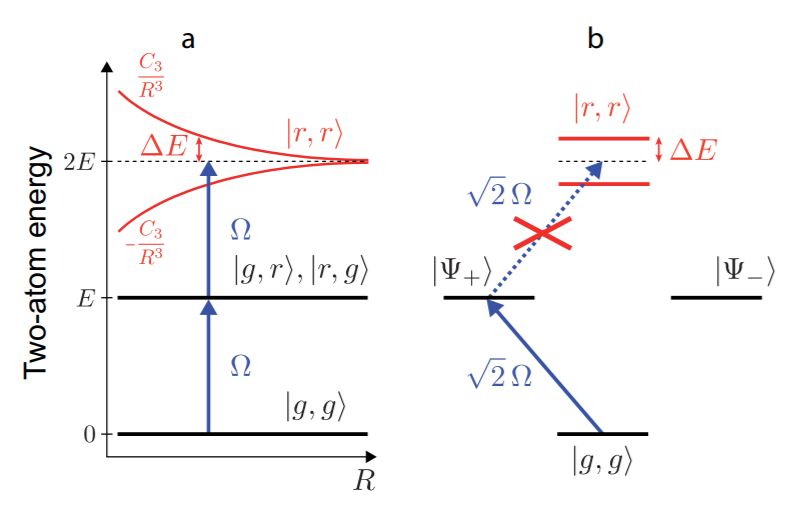
\includegraphics[height=0.32\textwidth,keepaspectratio]{rydbergblockadeeffect}
\caption{\label{fig:rydbergblockadeeffect} The Rydberg blockade effect. (a) The interaction between two atoms in Rydberg excited state $\ket{rr}$ as a function of $R$. When $V(R)>\Omega$ the laser is out of resonance with the shifted transition. (b) The energy level transition for the Rydberg blockade regime. The symmetric $\Delta E$ splitting from the non-interacting $\ket{rr}$ state and $\sqrt{N}\Omega$ coupling strength in the blockade regime is shown $^{[}$\citep{Gaetan2009ObservationRegime}$^{]}$.}
\end{figure}

The strong interaction between Rydberg atoms results in the Rydberg blockade effect which is useful for application of generating entanglement between systems. The blockade effect is shown in Fig.(\ref{fig:rydbergblockadeeffect}) where two atoms $A$ and $B$ are seperated a short-distance. The Rydberg states have a dipole-dipole interaction which scales as $V(R)\propto C_{3}/R^{3}$. When $R$>10 $\mu$m the long range van der Waals interaction scales as $V(R)=C_{6}/R^{6}$ where $C_{6}\approx C_{3}^{2}\approx n^{11}$ $^{[}$\citep{Gaetan2009ObservationRegime,Saffman2010QuantumAtoms}$^{]}$. 

When two non-interacting atoms are excited by a laser frequency which is resonant with $E/\hbar$ where $E$ is the energy splitting of ground $\ket{g}$ and Rydberg state $\ket{r}$ there are four possible connected states: $\ket{gg}$, $\ket{gr}$, $\ket{rg}$ and $\ket{rr}$. However, since Rydberg states have strong interactions this leads to a Rydberg-Rydberg interaction which result in the energy level shift such that state $\ket{rr}$ is no longer in resonance. When the atom separation is $\approx$<10 $\mu$ the blockade radius can be expressed as $^{[}$\citep{Comparat2010DipoleInvited}$^{]}$

\begin{equation}
\label{eq:bindingenergy}
R_{b}=\left ( \frac{C_{6}}{\hbar \Omega}^{1/6} \right ),
\end{equation}

for $V(R)>\Omega$ where the Rabi frequency is $Omega=(\vec{mu} \cdot \vec{E})/\hbar$. Therefore the Blockade effect results in excitation to the collective state $(\ket{gr}+\ket{rg})/\sqrt{2}$ where the enhance Rabi frequency is given as $\sqrt{N}Omega$. The Rydberg blockade effect can be used to complete a controlled phase gate where the phase of the target atom depends on the state of the control atom $^{[}$\citep{Urban2009ObservationTwoatoms}$^{]}$.  


\subsection{Quantum repeater architecture}
\begin{figure}[b]
\centering
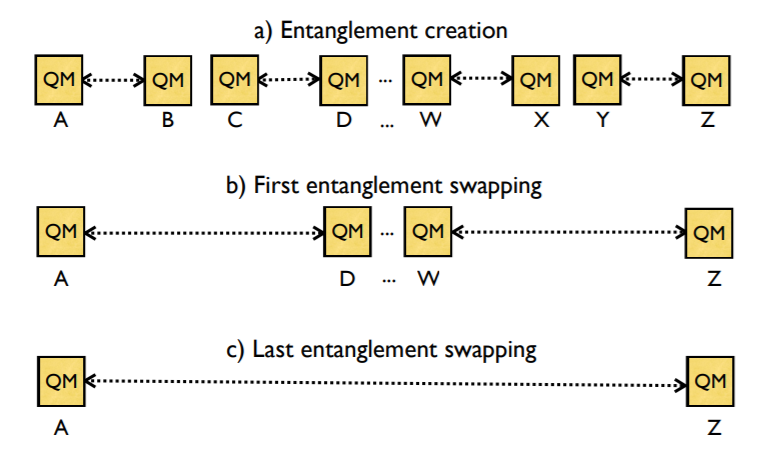
\includegraphics[height=0.25\textwidth,keepaspectratio]{entanglementswapping}
\caption{\label{fig:entanglementswapping} Quantum repeater scheme to distribute entanglement between quantum memory qubit A and Z through entanglement swapping $^{[}$\citep{Sangouard2011QuantumOptics}$^{]}$.}
\end{figure}
\noindent The four main requirements for long distance quantum communication are as follows $^{[}$\citep{Briegel1998QuantumCommunication,Muralidharan2016OptimalCommunication}$^{]}$:

\vspace{2mm}
\noindent (1) Generation of long distance entanglement.

 
\noindent (2) Polynomial resource and communication efficiency.


\noindent (3) A sufficiently long quantum memory.


\noindent (4) Sufficient suppression of loss and operational errors.
\vspace{2mm}
 
\noindent The earliest quantum repeater architecture is based on a one-dimensional line of length $L$ which is split in to sections of length  $L/M$ by memory qubits where $M$ is the number of memory nodes. Entanglement swapping between memory nodes is used to prepare long distance quantum state transfer. This repeater scheme is shown in Fig(\ref{fig:entanglementswapping}) where Bell state entanglement is initially generated between nearest neighbour quantum memories A-B,C-D,...W-X,Y-Z. Bell measurement of B-C,...X-Y followed by classically communicating the result to the other quantum memories produces entanglement between A-D,...W-Z $^{[}$\citep{Sangouard2011QuantumOptics}$^{]}$. This process is repeated until entanglement is generated between A and Z. Since entanglement is created probabilistically a heralded measurement is used to confirm the generation has been successful $^{[}$\citep{Chou2005Measurement-inducedEnsembles}$^{]}$.


The DLCZ protocol in Ref. [\citen{Duan2001Long-distanceOptics}] was developed in 2001 and is named after the initials of the paper co-authors. The DLCZ approach generates entanglement between atomic ensembles instead of between single atoms. The presented concept is collective excitation of atomic ensembles and Raman emission via an excited state. The benefit of collective encoding of atomic ensembles is discussed in detail in Section \ref{subsec:level1} and the resulting experimental research of collective excitation of Rydberg states is explored in Section \ref{subsec:level2}. The DLCZ protocol details the steps to generate entanglement between two atomic ensembles. Firstly, synchronized pumping of separated atomic ensembles where the emitted Stoke's photons are polarised and frequency filtered. Then the photons are directed at separate inputs of a 50-50 beam splitter. Finally Heralded measurement is completed where two detectors are placed at the outputs of the beam splitter. Protocol success is determined by a single detector click which prepares the entangled state $\ket{\Psi}=\frac{1}{\sqrt{2}}(\ket{0}\ket{1}+\ket{1}\ket{0})$. In Ref. [\citen{Duan2001Long-distanceOptics}] a polynomial increase in communication time as a function of distance is derived. However, the entangled state fidelity decreases polynomial with the number of quantum memories $^{[}$\citep{Sangouard2011QuantumOptics}$^{]}$. Entanglement swapping similarly uses Heralded measurement of ensemble B and C to entangle ensemble A and D where the measurement provides a form of entanglement purification. 

Recent quantum repeater proposals explore entanglement distillation and error correction protocols. Entanglement distillation prepares a small number of maximally entangled states from a large set of lower fidelity entangled states through entanglement purification schemes and local state operations $^{[}$\citep{Dur2007EntanglementCorrection,Muralidharan2016OptimalCommunication}$^{]}$. There are a number of different purification protocols outlined in Ref. [\citen{Dur2007EntanglementCorrection}] which utilise two-way classical communication to complete weak measurements, entanglement pumping and the recurrence protocol. Recurrence refers to joint operation followed by single state measurement after a previous successful single state measurement. 

Quantum error correction protocols rely on redundancy through encoding a logical qubit using a number of physical qubits. The combination of heralded entanglement generation and fault-tolerant preparation of logical states enables quantum error correction of entanglement swapping. However, this repeater architecture is also limited by the need for two-way classical communication Alternatively, if the loss and operational error rate is < 50 \%, physical qubits could be passed through an imperfect quantum channel using parity encoding. This protocol would remove the requirement for classical two-way communication to speed up the communication rate. However, recent repeater protocols remain experimentally challenging to implement due to experimental imperfections, the requirement for high fidelity quantum gate operation and large resource requirements $^{[}$\citep{Muralidharan2016OptimalCommunication,Ralph2005Loss-TolerantQubits}$^{]}$. 

